\documentclass[10pt,a4paper]{article}
\usepackage[utf8]{inputenc}
\usepackage{amsmath}
\usepackage{amsfonts}
\usepackage{mathtools}
\usepackage{amssymb}
\usepackage{graphicx}
\usepackage{subcaption}
\usepackage{dsfont}
\usepackage[strict]{changepage}
\usepackage{float}
\usepackage{parskip}
\makeatletter
\newcommand*{\transpose}{%
  {\mathpalette\@transpose{}}%
}
\newcommand*{\@transpose}[2]{%
  % #1: math style
  % #2: unused
  \raisebox{\depth}{$\m@th#1\intercal$}%
}

\author{Adam Jalkemo \texttt{adam@jalkemo.se} \and
Alexander Israelsson \texttt{israelsson.alexander@gmail.com} \and
Emil Westenius \texttt{emil@westenius.se} \and
Jonathan Andersson \texttt{mat11ja1@student.lu.se}}
\title{Adaptive Friction Compensation}
\begin{document}
\maketitle

\section{Introduction}
In this project a Furuta pendulum process will be used. The pendulum will be stabilized in the inverted position using a swing up controller and a top controller. When controlling the pendulum in the top position limit cycles will occur due to friction. By compensating for the friction we aim to stabilize the pendulum, the friction will be estimated using an adaptive method. To do this a Java controller and interface will be implemented and run on a linux/macOSX computer.
\section{Program structure}
For our suggested solution we will need one thread for the GUI and one for the controller. To communicate with the Furuta process we will use the analog box normally used during the control labs at LTH. The realtime package from Automatic Control at LTH will be used for communication in the GUI and controller implementation. It will be important to synchronize the controller calculations with the user inputs. A general overview can be seen in \ref{fig:uml}.
\begin{figure}
\centerline{
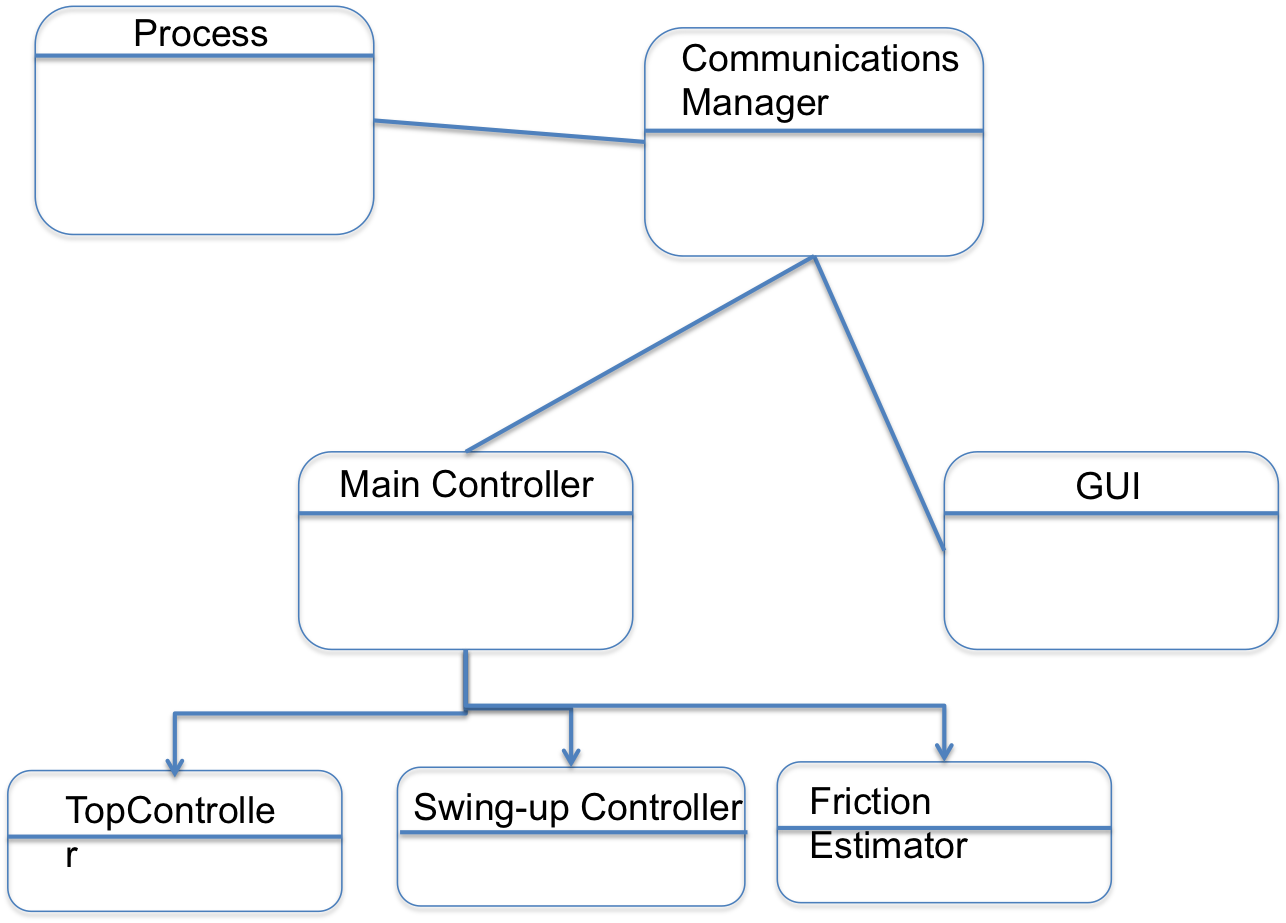
\includegraphics[scale=0.7]{umlfuruta.png}
}
\label{fig:uml}
\caption{Overview of the program structure}
\end{figure}
%% MORe STUFFS??

%ToDo UML AND DESCRIPTION OF CLASSES AND PACKAGES

\subsection{GUI}
The operator should be able to change controller parameters for both types of controller, the top controller and the swing up controller, as well as change the parameters for the friction estimation. 

The GUI will plot the outputs from the Furuta pendulum, the friction estimation, control signal, both uncompensated as well as the compensated signal. We aim to have different regressor modes for the friction compensation and the operator canl therefore change different parameters depending on the regressor chosen. 

We aim to be able to change all paramters on-line.

There will also be a start and stop button, these will start and stop the process. In the top left corner we will have a big X this will close the application. If you press "Share" you can share your results on Facebook, Twitter, Instagram and google+. This will lead to more time on the process, otherwise you will have to pay for each minute above 20 minutes a day. 

%Todo what parameters can be changed.

\subsection{Controller}
For the swing up a Lyapunov based controller will be used. In the top position a LQG controller will be used. The controllers will be implemented in Java.
Models for Coulomb and viscous friction and additional models for asymmetric friction will be considered. 

\section{Time plan}
\begin{table}[]
\centering
\caption{lolol}
\label{hoho}
\begin{tabular}{|l|l|l|}
\hline
Week & Description & Main Responsibility \\ \hline
13 & Hand in project plan & All members \\ \hline
& Begin GUI implementation & Adam \\ \hline
& Begin implementation of Java controller & Alexander \\ \hline
& Begin implementation of Matlab controller & Jonathan \\ \hline
& Research on friction estimator and model & Jonathan \\ \hline
14 & Working GUI implementation & Adam \\ \hline
& Write skeleton for report & Emil \\ \hline
& Working basic implementation of Java controller & Alexander \\ \hline
& Working basic implementation of Matlab controller & Jonathan \\ \hline
15 & Finished Matlab controller for tests & Jonathan \\ \hline
& & \\ \hline
& & \\ \hline
& & \\ \hline
& & \\ \hline
& & \\ \hline
& & \\ \hline
& & \\ \hline
& & \\ \hline
& & \\ \hline
17 & Predictive presentation 29/4 & \\ \hline
20 & Realtime presentation 19/5  & \\ \hline
\end{tabular}
\end{table}
The initial plan is handed in.


Start week 14, done week 15

\section{Responsibilities}
Theory
	What estimators to use
	What friction model
Friction controller in MATLAB
Controller in Java
	Friction
	Swingup
	Top controller
Program skeleton in java
GUI
Report
Presentation




\end{document}

